\documentclass[letterpaper,12pt]{article}
\setlength{\topmargin}{0in}
\setlength{\textheight}{9.0in}
\setlength{\textwidth}{6.5in}
\setlength{\columnsep}{0.25in}
\setlength{\headheight}{0in}
\setlength{\headsep}{0in}
\setlength{\oddsidemargin}{0.0in}
\setlength{\evensidemargin}{0.0in}
\setlength{\topskip}{0in}
\usepackage{times}
\usepackage{mdwlist}
\usepackage{hyperref}
\usepackage{array}
\usepackage{multicol}
\usepackage{multirow}
\usepackage{enumitem}
\usepackage{graphicx}
\usepackage{amsmath}
\usepackage{amsfonts}
\usepackage{algorithm2e}
\usepackage{parskip}
\usepackage{verbatim}
\hypersetup{colorlinks=true}
\renewcommand{\baselinestretch}{1.00}

\title{CSE 380 Project 2: Steady State Heat Equation Model Document}

\author{Sam Potter - STP663}

\begin{document}

\maketitle

\tableofcontents

\section{Abstract}
This document outlines the problem setup (governing equations and boundary conditions) as well as numerical solution techniques for solving 1D and 2D steady state heat equation problems using 2nd and 4th order finite difference.

\section{Executive Summary}
As of 12/14/18, there are still issues with convergence analysis. Due to this, while most tests can be performed, it is dubious to draw any conclusions because solver correctness has not been verified. Also, because much time was spent trying to fix solver convergence problems, \verb|PETSC| is not functioning.

Overall, I learned a great deal from this project and one of the most important lessons was the value of incremental development. Had I done a better job from the jump of adding and verifying functionality bit by bit, I think I could have avoided some of the traps and time sinks that have prevented me from completing all the deliverables for both Project 1 and Project 2

\section{Usage}
\subsection{Build Procedure}
\subsection{Autotools}
Autotools is used to compile the source code. The files \verb|configure.ac| and \verb|Makefile.am| are both setup to link to \verb|MASA|, \verb|GRVY|, and \verb|HDF5| and optionally \verb|PETSC| though functionality for the later seems broken. The \verb|Makefile.am| in \verb|src| is also modified with lines
\begin{verbatim}
AUTOMAKE_OPTIONS = foreign

if PETSC_ENABLED
	include $(PETSC_DIR)/lib/petsc/conf/variables
	AM_CXXFLAGS += -DINCLUDE_PETSC $(PETSC_CC_INCLUDES)
endif

bin_PROGRAMS = heatFD

heatFD_SOURCES = main.c utilities.c utilities.h

AM_CFLAGS = $(GRVY_CFLAGS)
AM_CFLAGS += $(MASA_CXXFLAGS)
AM_CFLAGS += $(HDF5_CFLAGS)
LIBS = $(GRVY_LIBS)
LIBS += $(MASA_LIBS)
LIBS += $(HDF5_LIBS)
LIBS += -lm

if PETSC_ENABLED
	heatFD_LDADD += ${PETSC_LIB}
endif
\end{verbatim}
A \verb|test| directory was created to perform regression tests using shell scripts and the \verb|make check| target, but convergence analysis issues (see below) have limited the number of regression tests to just working cases (as of 12/14/18, this is the 1d 2nd order case).

To facilitate troubleshooting, a shell script \verb|bootstrap.sh| can be sourced (very important to \verb|source| the script so environment variables are appropriately set in the parent process) to purge modules, then reload default \verb|TACC| modules, then depending on input either load modules for \verb|PETSC| or load a \verb|gcc| toolchain that has \verb|gcov|. The default behavior is to perform the later, while \verb|PETSC| linking can be accomplished by passing the option \verb|--petsc|. In all cases, the script sets necessary environment variables (\verb|PKGPATH|), then runs \verb|autoreconf -f -i| then \verb|./configure| with appropriate command line options. After that, user can run \verb|make| and \verb|make check| and optionally \verb|make coverage| if enabled.

\subsection{Coverage}
The \verb|gcov| and \verb|lcov| tools were used to evaluate how well the regression test suite created by the \verb|make check| target covered the use cases of the code. While the requirement is a minimum of 75\%, I was only able to achieve  approximately 30\% coverage (Fig. \ref{fig:cov}) because I did not include regression tests for the problem cases where my code was not achieving correct performance. While I could have written tests and most likely reached the 75\% mark, that would have been antithetical to the meaning of regression testing.

\begin{figure}[h]
\centering
\label{fig:cov}
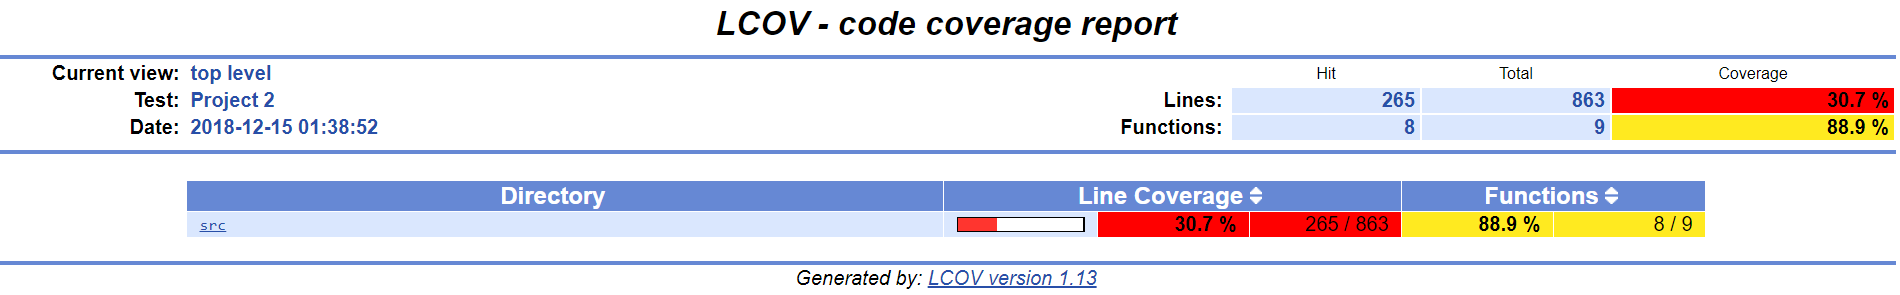
\includegraphics[width=1 \textwidth]{coverage.png}
\caption{Coverage report from lcov}
\end{figure}

\subsection{Continuous Integration}
In order to automate my regression testing, I used Travis-CI and a \verb|travis.yml| file to trigger a regression test build every time I pushed code to GitHub. I used the Docker image made available to the class as my base OS. I did have an issue getting Travis to work with my UTHPC repository, but was able to clone my repo into another repository under my own account and get the builds working (Fig. \ref{fig:travis}), so I don't know if this really counts.

\begin{figure}[h]
\centering
\label{fig:travis}
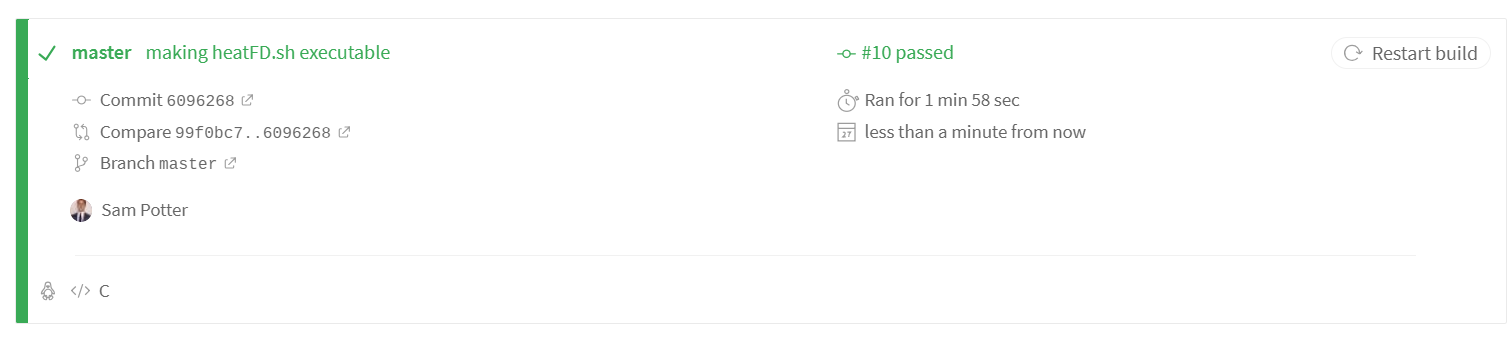
\includegraphics[width=1 \textwidth]{Travis.png}
\caption{Passing build from Travis-CI}
\end{figure}

\subsection{Input Options}
Input options available to the user are summarized in Table \ref{tab:input}.

\begin{table}[h]
\label{tab:input}
\caption{Application input options}
\begin{center}
\begin{tabular}{| c | c | c | c | }
\hline
option & description & acceptable range  \\ \hline \hline
method & iterative solver method & (Jacob,Gauss-Seidel)  \\ \hline
iter\_max & iterative solver max number of iterations & $>=1$ \\ \hline
tol & iterative solver convergence tolerance & positive real double  \\ \hline
order & finite difference order & (2,4)  \\ \hline
dimension & problem dimension & (1,2)   \\ \hline
kappa & material thermal conductivity & positive real double  \\ \hline
n & number of nodes along a side & $>2$  \\ \hline
Txmin & temperature at lower bound of x & real double  \\ \hline
Txmax & temperature at upper bound of x & real double  \\ \hline
Tymin & temperature at lower bound of y & real double  \\ \hline
Tymax & temperature at upper bound of y & real double  \\ \hline
Ax & MASA parameter Ax & real double  \\ \hline
By & MASA parameter By & real double  \\ \hline
verification & Bool switch: runn verification & (0=no, 1=yes)  \\ \hline
out\_mode & switch for output verbosity & (0=silent, 1=standard, 2=debug)  \\ \hline
timer & Bool switch: timing to stdout & (0=no, 1=yes)  \\ \hline
out\_file & file name to save results to & string  \\ \hline
\end{tabular}
\end{center}
\end{table}

\subsection{Verification Procedure}
To run the application in verification mode, the user can either set the value in the input file to 1 or pass the argument \verb|verification 1| on the command line. The user must also specify reasonable numbers for MASA parameters \verb|Ax| and \verb|By| in the input file based on domain size (assumed to be the unit interval in either $\mathbb{R}$ or $\mathbb{R}^2$). Output to \verb|stdout| includes problem details and L2 norm error with MASA exact solution.

\subsection{Verification Exercise}
\textbf{Outstanding issues with convergence results in all cases except 1D 2nd order}. See Fig \ref{fig:1d2nd}. through Fig. \ref{fig:2d2nd} for current results. Results for the 2D 4th order case are completely nonsensical. Note, using Gauss-Seidal iterative solver because Jacobi diverges for 4th order finite difference. This divergence stems from the fact that the system matrix $A$ is no longer strictly diagonally dominate, thus the Jacobi method won't converge with an arbitrary initial guess.

\begin{figure}[h]
\centering
\label{fig:1d2nd}
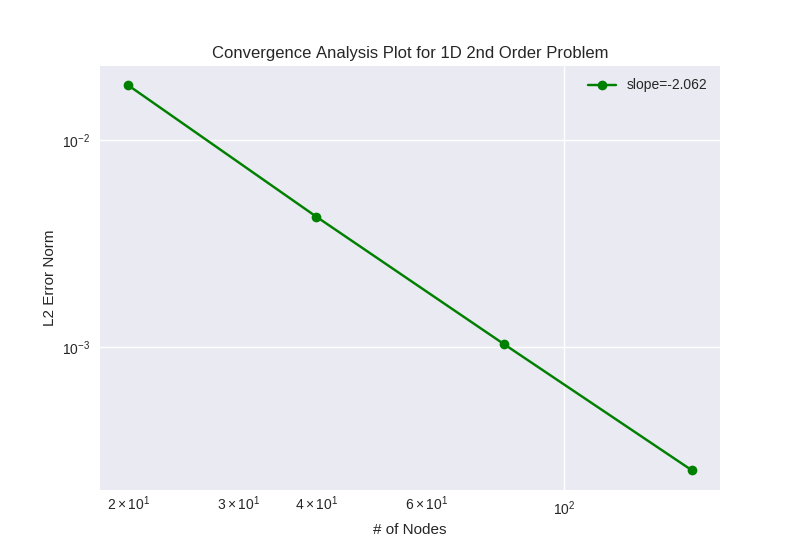
\includegraphics[width=1 \textwidth]{1d2nd.PNG}
\caption{Convergence results for 1D 2nd Order. Working as expected.}
\end{figure}

\begin{figure}[h]
\centering
\label{fig:1d4th}
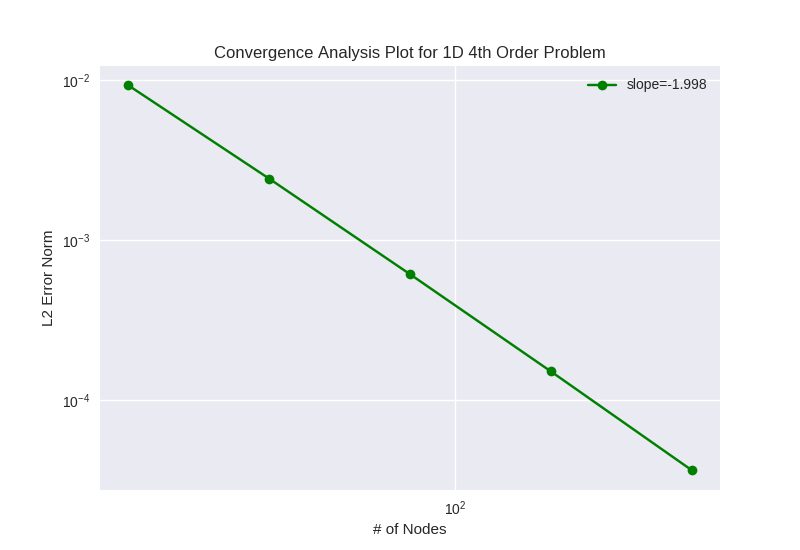
\includegraphics[width=1 \textwidth]{1d4th.PNG}
\caption{Convergence results for 1D 4th Order. Not working as expected. Convergence rate is half that of theoretical expectation.}
\end{figure}

\begin{figure}[h]
\centering
\label{fig:2d2nd}
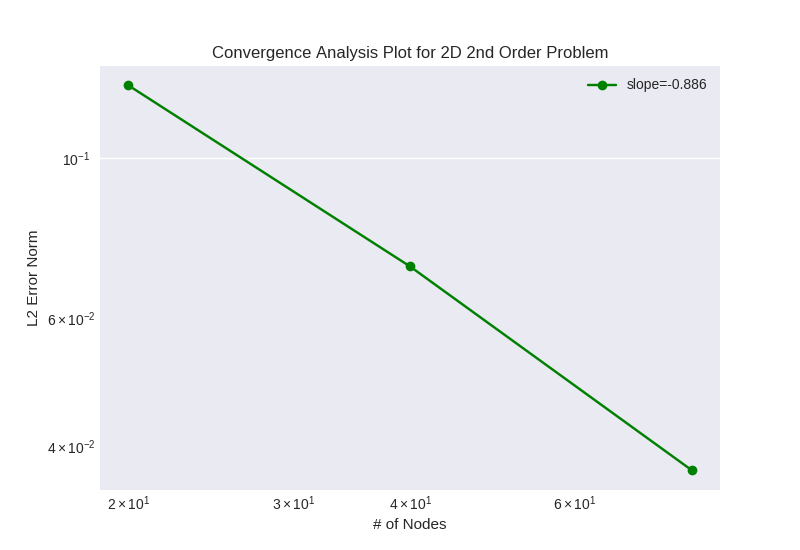
\includegraphics[width=1 \textwidth]{2d2nd.PNG}
\caption{Convergence results for 2D 2nd Order. Not working as expected. Convergence rate is half that of theoretical expectation.}
\end{figure}

\subsection{Performance Measures}
\textbf{Outstanding convergence issues in all cases except 1d 2nd order. Showing timing from 1 and 2d 2nd order}. As mentioned above, Gauss-Seidal method used. One dimensional results in Table \ref{tab:1Dtime}. Two dimensional results in Table \ref{tab:2Dtime}. Timings from \verb|PETSC| solves not available due to issues with compilation and linking.

\begin{table}[h]
\label{tab:1Dtime}
\caption{Timing results for 1D convergence testing w/ Gauss-Seidel}
\begin{center}
\begin{tabular}{| c | c | c | c || c |}
\hline
n &input &assemble &solve & total \\ \hline \hline
 20 &3.4e-3 &4.1e-3 &4.7e-4 & 1.4e-2\\ \hline
 40 &3.2e-2 &1.7e-3 &4.9e-3 & 4.3e-2\\ \hline
 80 &2.5e-2 &1.6e-3 &7.5e-2 & 1.1e-1\\ \hline
\end{tabular}
\end{center}
\end{table}

\begin{table}[h]
\label{tab:2Dtime}
\caption{Timing results for 2D convergence testing w/ Gauss-Seidel}
\begin{center}
\begin{tabular}{| c | c | c | c || c |}
\hline
n &input &assemble &solve & total \\ \hline \hline
 20 &7.1e-3 &5.3e-3 &9.3e-2 & 1.1e0\\ \hline
 40 &3.5e-3 &1.4e-2 &6.3e0 & 6.3e0\\ \hline
 80 &2.9e-3 &2.2e-1 &4.4e2 & 4.4e2\\ \hline
\end{tabular}
\end{center}
\end{table}

\section{Results}
\subsection{2D Plot}
I used Paraview to visualize my 2D solution. I wrote a short script in Python that used the \verb|h5py| library to read the HDF5 file and then write that data to an ASCII vtk file using a structured grid format. While I wouldn't say that the result is aesthetically beautiful it is beautiful in the sense that it shows that I clearly have either a boundary value issue somewhere or an issue with how I've ordered my solution vector (Fig. \ref{fig:2dplot}). This kind of information will be helpful as I continue to debug.

\begin{figure}[h]
\centering
\label{fig:2dplot}
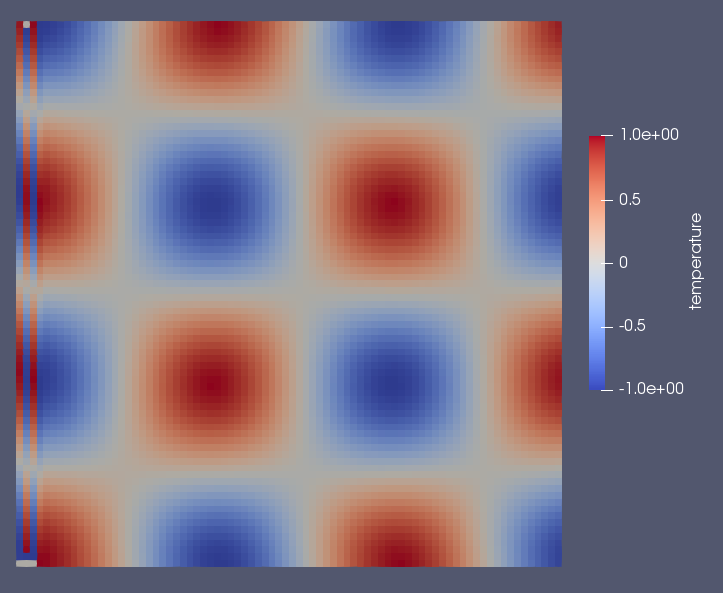
\includegraphics[width=.8 \textwidth]{2dplot.PNG}
\caption{Plot of scalar temperature field for a 2D MASA verification problem. 80 nodes used in the finite difference solution.}
\end{figure}

\subsection{1D Plot}
Finally, while not a required deliverable, I wanted to show a plot of my 1d 4th order solution with 80 nodes (Fig. ) because it seems to match the analytical solution well, but I'm still getting slow convergence. This tells me something may be going on in how I'm calculating the L2 error. I am continuing to hunt this issue down.

\begin{figure}[h]
\centering
\label{fig:1dplot}
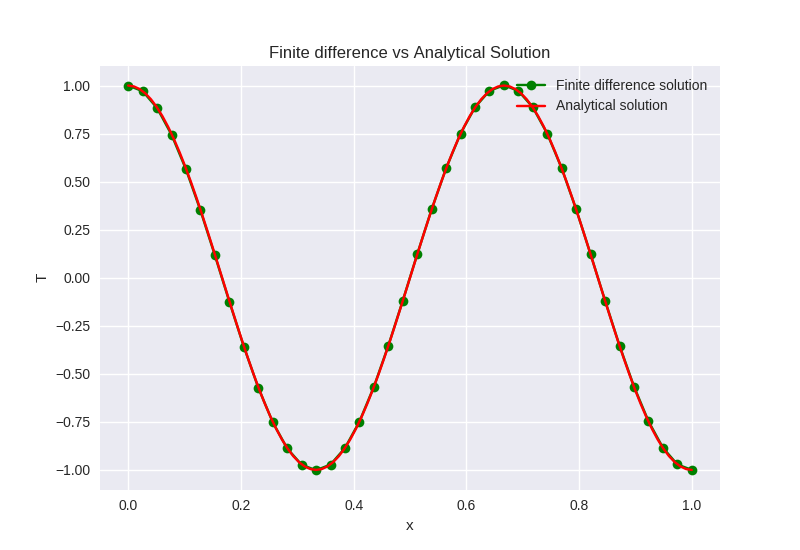
\includegraphics[width=1 \textwidth]{1d4th_soln.png}
\caption{Plot of scalar temperature field for a 1D MASA verification problem. 80 nodes used in the finite difference solution.}
\end{figure}

\section{Problem Setup}
\subsection{Governing Equations}
\subsubsection{One Dimensional Case}
In one dimension, the governing equation is
\begin{equation}
\label{gov1}
-k \frac{\partial^2 T(x)}{\partial x^2} = q(x)
\end{equation}
\subsubsection{Two Dimensional Case}
In two dimensions, the governing equation is
\begin{equation}
\label{gov2}
-k \nabla^2 T(x,y) = q(x,y)
\end{equation}
\subsection{Nomenclature}
\subsubsection{One Dimensional Case}
\begin{itemize}
\item $q(x)$: Heat flux at spatial coordinate location $x$
\item $x$: Spatial coordinate in 1D
\item $T(x)$: Temperature of material at spatial coordinate location $x$
\item $k$: Material thermal conductivity
\end{itemize}
\subsubsection{Two Dimensional Case}
\begin{itemize}
\item $q(x,y)$: Heat flux at spatial coordinate location $(x,y)$
\item $x$: Spatial coordinate in first dimension.
\item $y$: Spatial coordinate in second dimension
\item $T(x,y)$: Temperature of material at spatial coordinate location $(x,y)$
\item $k$: Material thermal conductivity
\item $\nabla$: Gradient operator in 2D Cartesian coordinates
\end{itemize}
\subsection{Boundary Conditions}
\subsubsection{One Dimensional Case}
\begin{itemize}
\item $T(x=0)$: \textbf{Required:} Temperature at spatial location $x=0$.
\item $T(x=1)$: \textbf{Required:} Temperature at spatial location $x=1$. 
\item $q(x)$: \textbf{Optional:} Heat flux at spatial coordinate location $x$
\end{itemize}
\subsubsection{Two Dimensional Case}
\begin{itemize}
\item $T(x=0, y)$: \textbf{Required:} Temperature at spatial boundary $(x=0, y)$.
\item $T(x=1, y)$: \textbf{Required:} Temperature at spatial boundary $(x=1, y)$. 
\item $T(x, y=0)$: \textbf{Required:} Temperature at spatial boundary $(x, y=0)$.
\item $T(x, y=1)$: \textbf{Required:} Temperature at spatial boundary $(x, y=1)$.  
\item $q(x, y)$: \textbf{Optional:} Heat flux at spatial coordinate location $(x, y)$
\end{itemize}
\subsection{Constitutive Inputs}
\subsubsection{One Dimensional Case}
\begin{itemize}
\item $k$: \textbf{Required:} Material thermal conductivity. Assumed homogeneous across the material domain
\end{itemize}
\subsubsection{Two Dimensional Case}
\begin{itemize}
\item $k$ \textbf{Required:} Material thermal conductivity. Assumed homogeneous across the material domain
\end{itemize}

\section{Assumptions}
\subsection{One Dimensional Case}
\begin{itemize}
\item The problem domain is on the interval $\Omega =  x \in [0, 1]$.
\item The boundary conditions are restricted to Dirichlet types, i.e. only temperature can be specified at the domain boundaries, not heat flux.
\item Further, these Dirichlet boundary conditions are given, i.e. temperature at mesh nodes on the boundary are specified
\item The material thermal conductivity is constant over the domain
\item Mesh step size ($\Delta x = h$) is uniform, i.e. no refinement near boundaries, source terms, etc.
\end{itemize}
\subsection{Two Dimensional Case}
\begin{itemize}
\item The problem domain is the unit square $ \Omega = (x,y) \in [0, 1] \times [0,1]$
\item The boundary conditions are restricted to Dirichlet types, i.e. only temperature can be specified at the domain boundaries, not heat flux.
\item Further, these Dirichlet boundary conditions are given, i.e. temperature at mesh nodes on the boundary are specified
\item The material thermal conductivity is constant over the domain
\item Mesh step size ($\Delta x = \Delta y = h$) is uniform, i.e. no refinement near boundaries, source terms, etc.
\end{itemize}

\section{Numerics}
\subsection{Finite Difference}
\subsubsection{One Dimensional Case}
\textbf{2nd Order Finite Difference in One Dimension}
\begin{equation}
\label{1D2FD}
\frac{\partial^2 T(x)}{\partial x^2} = \frac{T(x_{i+1}) - 2  T(x_i) + T(x_{i-1})}{\Delta x^2} - \frac{\Delta x^2}{12} \frac{\partial ^4 T(x)}{\partial x^4} |_{x_i} + ...
\end{equation}
\textbf{Expansion of 1D Heat Equation with 2nd Order Finite Difference}
\begin{equation}
\label{heat1d2FD}
-k \frac{T(x_{i+1}) - 2  T(x_i) + T(x_{i-1})}{\Delta x^2} = q(x_i)
\end{equation}
\textbf{4th Order Finite Difference in One Dimension}
\begin{equation}
\label{1D4FD}
\frac{\partial^2 T(x)}{\partial x^2} = \frac{-T(x_{i+2}) + 16  T(x_{i+1}) - 30T(x_i) + 16 T(x_{i-1}) -T(x_{i-2})}{12 \Delta x^2} - \frac{\Delta x^4}{90} \frac{\partial ^6 T(x)}{\partial x^6} |_{x_i} + ...
\end{equation}
\textbf{Expansion of 1D Heat Equation with 4th Order Finite Difference}
\begin{equation}
\label{heat1d4FD}
-k \frac{-T(x_{i+2}) + 16  T(x_{i+1}) - 30T(x_i) + 16 T(x_{i-1}) -T(x_{i-2})}{12 \Delta x^2} = q(x_i)
\end{equation}
\subsubsection{Two Dimensional Case}
Finite difference formulas for the second order partial derivatives are the same as in the 1D case. The difference is that there are now two of the terms (one for each spatial direction) in the discrete form of the governing equation

\textbf{2D Heat Equation with 2nd Order Finite Difference}
\begin{multline}
\label{heat2d2FD}
-k \Big( \frac{T(x_{i+1}, y_j) - 2  T(x_i, y_j) + T(x_{i-1}, y_j)}{\Delta x^2} + \\ \frac{T(x_i,y_{j+1}) - 2  T(x_i, y_j) + T(x_i, y_{j-1})}{\Delta y^2} \Big)= q(x_i, y_i)
\end{multline}
\textbf{2D Heat Equation with 4th Order Finite Difference}
\begin{multline}
\label{heat2d4FD}
-k \Big(\frac{-T(x_{i+2}, y_j) + 16  T(x_{i+1}, y_j) - 30T(x_i, y_j) + 16 T(x_{i-1}, y_j) -T(x_{i-2}, y_j)}{12 \Delta x^2} + \\ \frac{-T(x_i, y_{j+2}) + 16  T(x_i, y_{j+1}) - 30T(x_i, y_j) + 16 T(x_i, y_{j-1}) -T(x_i, y_{j-2})}{12 \Delta y^2} \Big) = q(x_i, y_j)
\end{multline}
\subsection{Meshing}
\subsubsection{General Notes}
\begin{itemize}
\item Mesh is grid based
\end{itemize}
\subsubsection{1D Problem}
Mesh and finite difference stencil details can be found in Fig. \ref{1DMesh}

\begin{figure}[h]
\centering
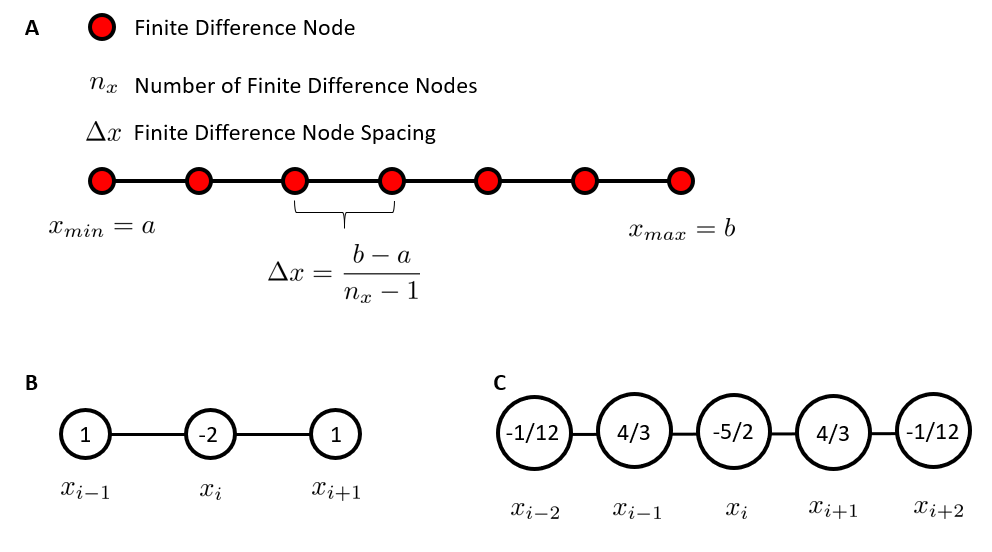
\includegraphics[width=1 \textwidth]{1D_Mesh.PNG}
\caption{Finite difference mesh and stencil details for the 1D Heat Equation problem. A) Mesh details. B) Stencil for 2nd order finite difference. C) Stencil for 4th order finite difference.}
\label{1DMesh}
\end{figure}
\subsubsection{2D Problem}
Mesh details can be found in Fig. \ref{2DMesh}

\begin{figure}[h]
\centering
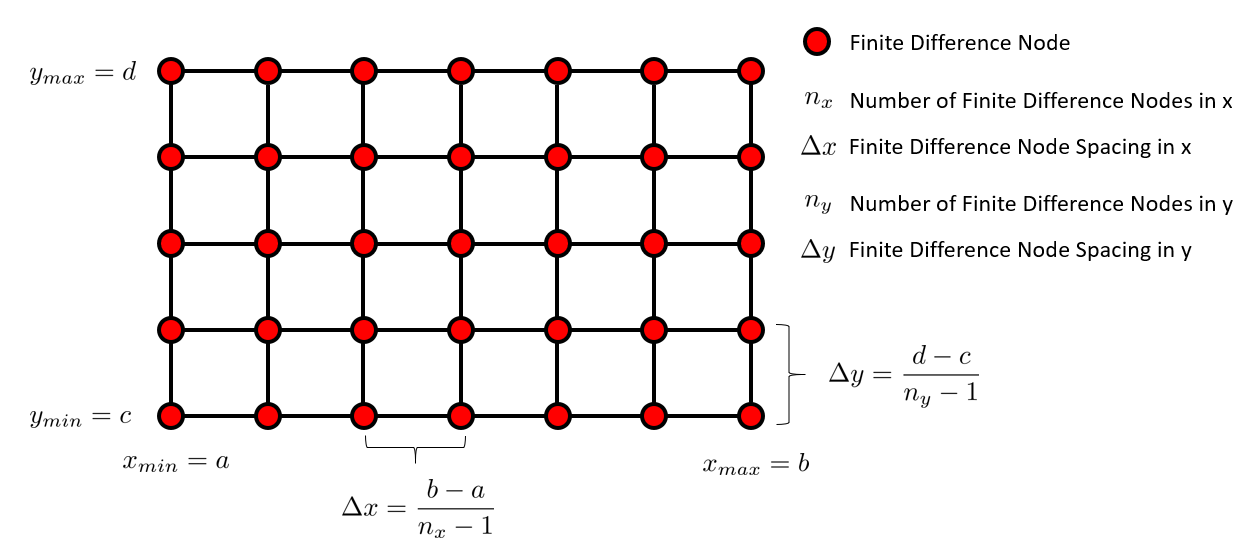
\includegraphics[width=1 \textwidth]{2D_Mesh.PNG}
\caption{Finite difference mesh details for the 2D Heat Equation problem.}
\label{2DMesh}
\end{figure}

Finite difference stencil details can be found in Fig. \ref{2DStencil}

\begin{figure}[h]
\centering
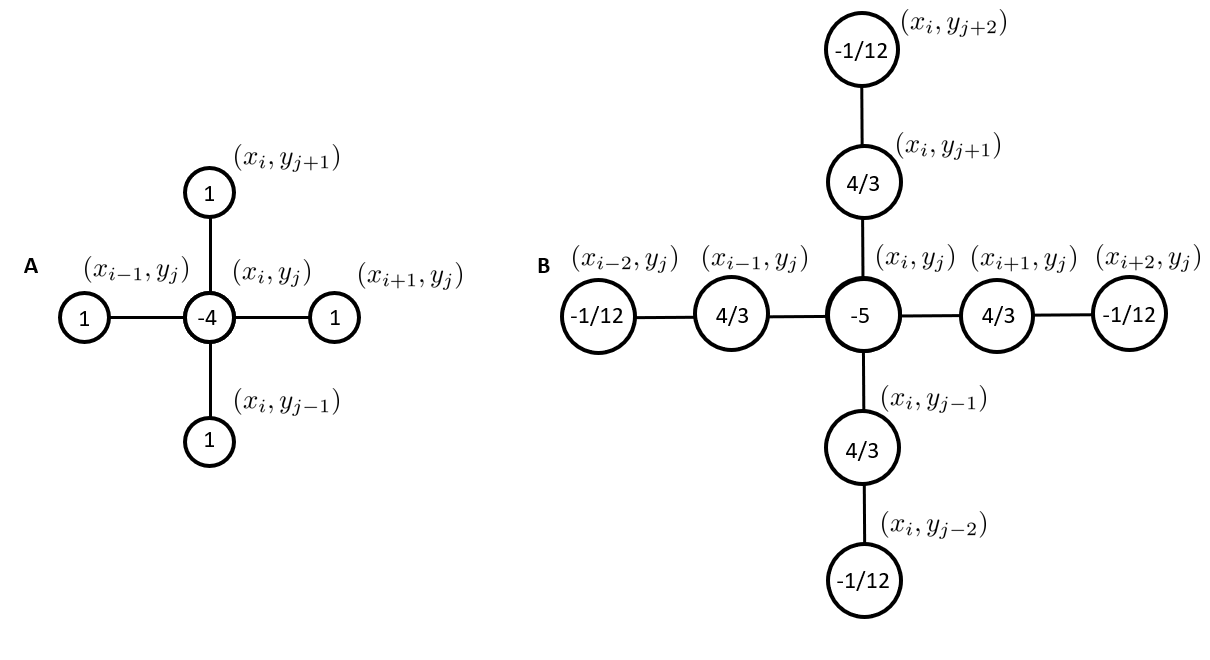
\includegraphics[width=1 \textwidth]{2D_Stencil.PNG}
\caption{Finite difference mesh details for the 2D Heat Equation problem.}
\label{2DStencil}
\end{figure} 
\subsection{Linear System}
\subsubsection{1D Problem}
\textbf{2nd Order Finite Difference} The resulting system of equations has the form
\begin{align}
\label{1D2FDsys}
2 T(x_1) - T(x_2) &= \frac{h^2}{k} (q(x_1)) + T(x_0) \\
-T(x_1) + 2 T(x_2) - T(x_3) &= \frac{h^2}{k} q(x_2) \\
\vdots \\
2 T(x_{n_x - 1}) - T(x_{n_x - 2}) &= \frac{h^2}{k} (q(x_{n_x - 1})) + T(x_{n_x}) \\
\end{align}
The resulting matrix equation is $AT = Q$ with $A \in \mathbb{R}^{n_xn_y \times n_xn_y}$ given by the matrix
\[
A=
\begin{bmatrix}
2 & -1 & 0 & 0 & \dots &  & 0 \\
-1 & 2 & -1 & 0 & \dots &  & 0\\
0 & -1 & 2 & -1 & 0 & \dots & 0 \\
\vdots &  & \ddots & \ddots & \ddots & & 0 \\
 & & & -1 & 2 & -1 & 0 \\
0 & \dots & \dots & 0 & -1 & 2 & -1 \\
0 & \dots & \dots & \dots & 0 & -1 & 2 \\
\end{bmatrix}
\]
and the RHS vector, $Q \in \mathbb{R}^{n_x}$ by
\[
Q= 
\begin{bmatrix}
\frac{h^2}{k} q(x_1) + T(x_0) \\
\frac{h^2}{k} q(x_2) \\
\vdots \\
\frac{h^2}{k} q(x_{n_x-2}) \\
\frac{h^2}{k} q(x_{n_x-1}) + T(x_{n_x})
\end{bmatrix}
\]
The sparsity of the matrix $A$ is visualized in Fig. \ref{1D2ndSparse}. There are typically 3 non-zero entries for a interior element row

\begin{figure}[h]
\centering
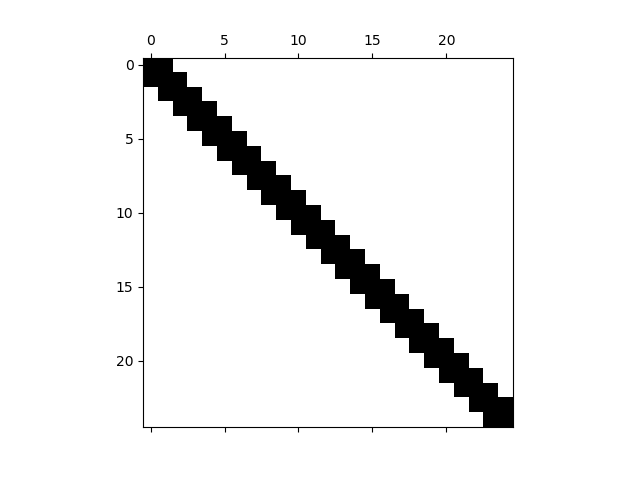
\includegraphics[width=.9 \textwidth]{oned_sparse_2.png}
\caption{Sparsity of problem system in 1D and 2nd order finite difference for an example 25 degrees of freedom system. Blocks in black indicate non-zero entries}
\label{1D2ndSparse}
\end{figure} 

\textbf{4th Order Finite Difference} The resulting system of equations has the form
\begin{align}
\label{1D4FDsys}
2 T(x_1) - T(x_2) &= \frac{h^2}{k} (q(x_1)) + T(x_0) \nonumber \\
 - \frac{4}{3} T(x_{1}) +\frac{5}{2} T(x_2) -\frac{4}{3} T(x_{3})  + \frac{1}{12} T(x_4) &= \frac{h^2}{k} (q(x_2)) - \frac{1}{12} T(x_0) \nonumber \\
\frac{1}{12} T(x_1) -\frac{4}{3} T(x_{2}) +\frac{5}{2} T(x_3) - \frac{4}{3} T(x_{4}) + \frac{1}{12} T(x_5) &= \frac{h^2}{k} q(x_3) \nonumber \\
\vdots \\
\frac{1}{12} T(x_{n_x - 5}) -\frac{4}{3} T(x_{n_x - 4}) +\frac{5}{2} T(x_{n_x - 3}) - \frac{4}{3} T(x_{n_x - 2}) + \frac{1}{12} T(x_{n_x - 1}) &= \frac{h^2}{k} q(x_{n_x - 3}) \nonumber \\
-\frac{4}{3} T(x_{n_x - 3}) +\frac{5}{2} T(x_{n_x - 2}) - \frac{4}{3} T(x_{n_x - 1}) + \frac{1}{12} T(x_{n_x - 4}) &= \frac{h^2}{k} (q(x_{n_x - 2})) - \frac{1}{12} T(x_{n_x}) \nonumber \\
2 T(x_{n_x - 1}) - T(x_{n_x - 2}) &= \frac{h^2}{k} (q(x_{n_x - 1})) + T(x_{n_x}) \nonumber \\ \nonumber
\end{align}
where second order finite difference approximations are used on the first interior boundary nodes to deal with the fact that in those locations the 4th order approximations require information from nodes that do not exist. 

The resulting linear system of equations is $AT = Q$ with $A \in \mathbb{R}^{n_xn_y \times n_xn_y}$ given by the matrix
\[
A=
\begin{bmatrix}
2 & -1 & 0 & 0 & \dots & & & 0 \\
-\frac{4}{3} & \frac{5}{2} & -\frac{4}{3} & \frac{1}{12} & 0 & \dots & & 0\\
\frac{1}{12} & -\frac{4}{3} & \frac{5}{2} & -\frac{4}{3} & \frac{1}{12} & 0 & \dots & 0 \\
0 & \frac{1}{12} & -\frac{4}{3} & \frac{5}{2} & - \frac{4}{3} & \frac{1}{12} & 0 & \vdots \\
\vdots &  & \ddots & \ddots & \ddots & \ddots & \ddots & \\
0 & \dots & 0 & \frac{1}{12} & -\frac{4}{3} & \frac{5}{2} & -\frac{4}{3} & \frac{1}{12} \\
0 & \dots & \dots & 0 & \frac{1}{12} & -\frac{4}{3} & \frac{5}{2} & -\frac{4}{3} \\
0 & \dots & & & \dots & 0 & -1 & 2 \\
\end{bmatrix}
\]
and the RHS vector, $Q \in \mathbb{R}^{n_x}$ by
\[
Q= 
\begin{bmatrix}
\frac{h^2}{k} q(x_1) + T(x_0) \\
\frac{h^2}{k} q(x_2) - \frac{1}{12} T(x_0)\\
\frac{h^2}{k} q(x_3) \\
\vdots \\
\frac{h^2}{k} q(x_{n_x - 3}) \\
\frac{h^2}{k} q(x_{n_x-2}) - \frac{1}{12} T(x_{n_x}) \\
\frac{h^2}{k} q(x_{n_x-2}) + T(x_{n_x})
\end{bmatrix}
\]
The sparsity of the matrix $A$ is visualized in Fig. \ref{1D4thSparse}. There are typically 5 non-zero entries for a interior element row 

\begin{figure}[h]
\centering
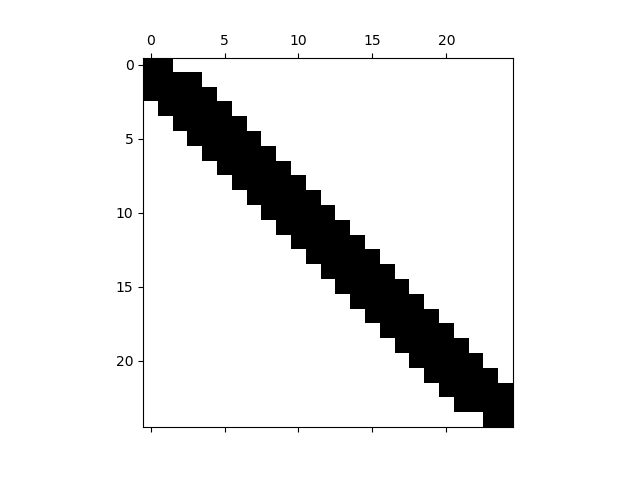
\includegraphics[width=.9 \textwidth]{oned_sparse_4.png}
\caption{Sparsity of problem system in 1D and 4th order finite difference for an example 25 degrees of freedom system. Blocks in black indicate non-zero entries}
\label{1D4thSparse}
\end{figure}

\subsubsection{2D Problem}
\textbf{2nd Order Finite Difference} The resulting system of equations has the form (stepping through $x$ first) and is a simple extension of the 1D problem.
\begin{align}
\label{2D2FDsys}
4 T(x_1, y_1) - T(x_2, y_1) &= \frac{h^2}{k} (q(x_1, y_1)) + T(x_0, y_1) \nonumber \\
-T(x_1, y_1) + 4 T(x_2, y_1) - T(x_3, y_1) &= \frac{h^2}{k} q(x_2, y_1) \nonumber \\
\vdots \nonumber \\
4 T(x_{n_x - 1}, y_1) - T(x_{n_x - 2}, y_1) &= \frac{h^2}{k} (q(x_{n_x - 1}, y_1)) + T(x_{n_x}, y_1)  \\
\vdots \nonumber \\
4 T(x_1, y_2) - T(x_2, y_2) &= \frac{h^2}{k} (q(x_1, y_2)) + T(x_0, y_2) \nonumber \\
\vdots \nonumber \\
4 T(x_{n_x - 1}, y_2) - T(x_{n_x - 2}, y_2) &= \frac{h^2}{k} (q(x_{n_x - 1}), y_2) + T(x_{n_x}, y_2) \nonumber
\end{align}
The resulting linear system of equations is $AT = Q$ with $A \in \mathbb{R}^{n_xn_y \times n_xn_y}$ given by the block, tridiagonal matrix
\[
A = 
\begin{bmatrix}
S & -I & &\\
-I & S & -I & \\
 & -I & S & -I \\
 & & \ddots & \ddots & \ddots \\
 & & & -I & S & -I \\
 & & & & -I & S
\end{bmatrix}
S \in \mathbb{R}^{n_x \times n_x} =
\begin{bmatrix}
4 & -1 & 0 & 0 & \dots &  & 0 \\
-1 & 4 & -1 & 0 & \dots &  & 0\\
0 & -1 & 4 & -1 & 0 & \dots & 0 \\
\vdots &  & \ddots & \ddots & \ddots & & 0 \\
 & & & -1 & 4 & -1 & 0 \\
0 & \dots & \dots & 0 & -1 & 4 & -1 \\
0 & \dots & \dots & \dots & 0 & -1 & 4 \\
\end{bmatrix}
\]
and $I$ is the identity matrix in $\mathbb{R}^{n_x \times n_x}$.
The RHS vector, $Q \in \mathbb{R}^{n_x n_y}$ is
\[
Q= 
\begin{bmatrix}
\frac{h^2}{k}q(x_1, y_1) + T(x_0, y_1) \\
\frac{h^2}{k}q(x_2, y_1) \\
\vdots \\
\frac{h^2}{k}q(x_{n_x-2}, y_1) \\
\frac{h^2}{k}q(x_{n_x-1}, y_1) + T(x_{n_x}, y_1) \\
\vdots
\frac{h^2}{k}q(x_1, y_1) + T(x_0, y_2) \\
\frac{h^2}{k}q(x_2, y_2) \\
\vdots \\
\frac{h^2}{k}q(x_{n_x-2}, y_2) \\
\frac{h^2}{k}q(x_{n_x-1}, y_2) + T(x_{n_x}, y_2) \\
\end{bmatrix}
\]
The sparsity of the matrix $A$ is visualized in Fig. \ref{2D2ndSparse}. There are typically 5 non-zero entries for a interior element row
 
\begin{figure}[h]
\centering
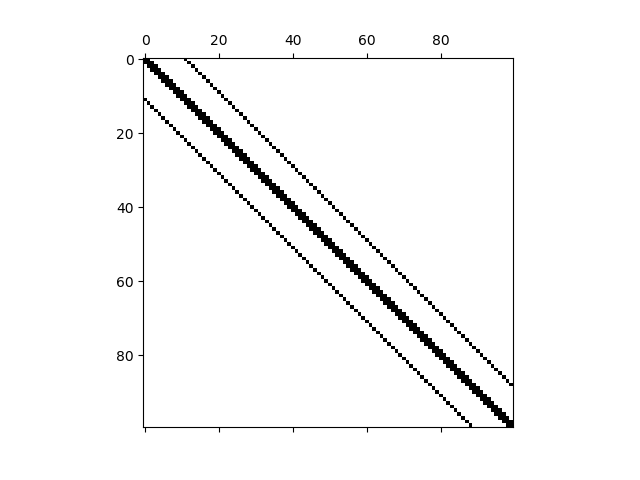
\includegraphics[width=.9 \textwidth]{twod_sparse_2.png}
\caption{Sparsity of problem system in 2D and 2nd order finite difference for an example 10 x 10 degrees of freedom system. Blocks in black indicate non-zero entries}
\label{2D2ndSparse}
\end{figure}

\textbf{4th Order Finite Difference} As in the 2nd order case, the resulting system of equations has form that is a simple extension of the 1D problem.
The resulting linear system of equations is $AT = Q$ with $A \in \mathbb{R}^{n_xn_y \times n_xn_y}$ given by the block, tridiagonal matrix
\[
A = 
\begin{bmatrix}
S & -I & &\\
-I & S & -I & \\
 & -I & S & -I \\
 & & \ddots & \ddots & \ddots \\
 & & & -I & S & -I \\
 & & & & -I & S
\end{bmatrix}
S \in \mathbb{R}^{n_x \times n_x} =
\begin{bmatrix}
4 & -1 & 0 & 0 & \dots & & & 0 \\
-\frac{4}{3} & 5 & -\frac{4}{3} & \frac{1}{12} & 0 & \dots & & 0\\
\frac{1}{12} & -\frac{4}{3} & 5 & -\frac{4}{3} & \frac{1}{12} & 0 & \dots & 0 \\
0 & \frac{1}{12} & -\frac{4}{3} & 5 & - \frac{4}{3} & \frac{1}{12} & 0 & \vdots \\
\vdots &  & \ddots & \ddots & \ddots & \ddots & \ddots & \\
0 & \dots & 0 & \frac{1}{12} & -\frac{4}{3} & 5 & -\frac{4}{3} & \frac{1}{12} \\
0 & \dots & \dots & 0 & \frac{1}{12} & -\frac{4}{3} & 5 & -\frac{4}{3} \\
0 & \dots & & & \dots & 0 & -1 & 4 \\
\end{bmatrix}
\]
and $I$ is the identity matrix in $\mathbb{R}^{n_x \times n_x}$.
The RHS vector, $Q \in \mathbb{R}^{n_x n_y}$ is
\[
Q= 
\begin{bmatrix}
\frac{h^2}{k}q(x_1, y_1) + T(x_0, y_1) \\
\frac{h^2}{k}q(x_2, y_1) - \frac{1}{12} T(x_0, y_1)\\
\frac{h^2}{k}q(x_3, y_1) \\
\vdots \\
\frac{h^2}{k}q(x_{n_x - 3}, y_1) \\
\frac{h^2}{k}q(x_{n_x-2}, y_1) - \frac{1}{12} T(x_{n_x}, y_1) \\
\frac{h^2}{k}q(x_{n_x-2}, y_1) + T(x_{n_x}, y_1) \\
\frac{h^2}{k}q(x_1, y_2) + T(x_0, y_2) \\
\frac{h^2}{k}q(x_2, y_2) - \frac{1}{12} T(x_0, y_2)\\
\frac{h^2}{k}q(x_3, y_2) \\
\vdots \\
\frac{h^2}{k}q(x_{n_x - 3}, y_2) \\
\frac{h^2}{k}q(x_{n_x-2}, y_2) - \frac{1}{12} T(x_{n_x}, y_2) \\
\frac{h^2}{k}q(x_{n_x-2}, y_2) + T(x_{n_x}, y_2)
\end{bmatrix}
\]
The sparsity of the matrix $A$ is visualized in Fig. \ref{2D4thSparse}. There are typically 7 non-zero entries for a interior element row

\begin{figure}[h]
\centering
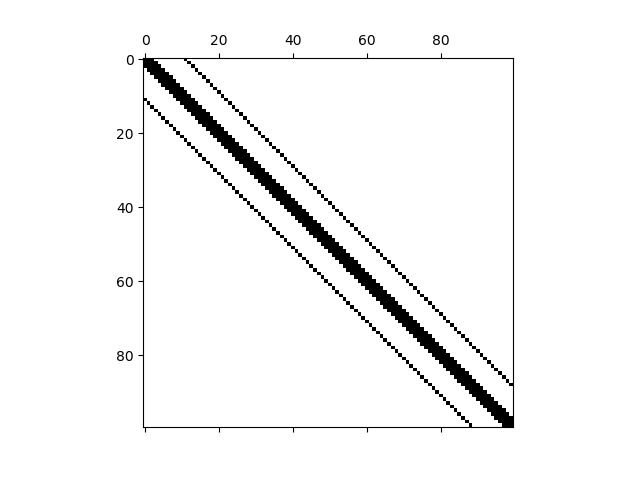
\includegraphics[width=.9 \textwidth]{twod_sparse_4.png}
\caption{Sparsity of problem system in 2D and 4th order finite difference for an example 10 x 10 degrees of freedom system. Blocks in black indicate non-zero entries}
\label{2D4thSparse}
\end{figure}

\subsection{Solvers}
\subsubsection{Jacobi}
\textbf{Algorithm Outline}
Given $Ax=B$, decompose $A$ into $A = D + R$ with $D$ being the diagonal and $R$ the off diagonal terms. Solve for next iterative guess of $x$ via
\begin{equation}
\label{Jacobi}
x^{k+1} = D^{-1} (b - Rx^k)
\end{equation}
and terminate when difference norm term $||x^{k} - x^{k-1}||$ falls below user specified tolerance $\epsilon$. User must also specify an initial guess $x^0$.

\textbf{Psuedo-Code}

\begin{algorithm}[H]
$k = 0$\;
error = $||b - A x^{(k)}||_2$ \;
\While{error $>$ epsilon}{
\For{$i=1$ \KwTo $n$}{
$\sigma = 0$\;
\For{$j=1$ \KwTo n}{
\If{$j \neq i$}{
$\sigma = \sigma + a_{ij} x_j^{(k)}$\;
}
}
$x_i^{(k+1)} = \frac{1}{a_{ii}} (b_i - \sigma)$ \;
}
$k = k + 1$ \;
error = $||b - A x^{(k+1)}||_2$ \;
} 
\end{algorithm}

\subsubsection{Gauss-Seidel}
\textbf{Algorithm Outline}
Given $Ax=B$, decompose $A$ into $A = L + R$ with $L$ being lower triangular and $U$ upper triangular. Solve for next iterative guess of $x$ via
\begin{equation}
\label{Gauss-Seidal}
x^{k+1} = L^{-1} (b - Ux^k)
\end{equation}
and terminate when difference norm term $||x^{k} - x^{k-1}||$falls below user specified tolerance $\epsilon$. Note, this method only requires storage of a single vector sized to the number of variables, whereas the Jacobi requires storage of two such vecotrs. User must also specify an initial guess $\phi$.

\textbf{Psuedo-Code}

\begin{algorithm}[H]
error = $||b - A \phi||_2$ \;
\While{error $>$ epsilon}{
\For{$i=1$ \KwTo $n$}{
$\sigma = 0$\;
\For{$j=1$ \KwTo n}{
\If{$j \neq i$}{
$\sigma = \sigma + a_{ii} \phi_j$\;
}
}
$\phi_i = \frac{1}{a_{ii}} (b_i - \sigma)$ \;
}
error = $||b - A \phi||_2$ \;
} 
\end{algorithm}
\subsection{Memory Considerations}
A conservative memory estimate would be to calculate the memory required to store each element of the matrix $A$ and vectors $T, Q$ in double precision floating point as a function of the problem size. Count the $T$ vector twice to accommodate the need to store two of these vectors if using Jacobi solution method. Note, the storage could be vastly improved if matvec storage is used for $A$.

\subsubsection{1D Problem}
\begin{itemize}
\item $A$: $n_x \times n_x$ floating point numbers
\item $Q$: $n_x$ floating point numbers
\item $T$: $n_x$ floating point numbers
\end{itemize}
\textbf{Total Floating Point Numbers:} $n_x^2 + 3 n_x$

\textbf{Memory estimation:} $64 \text{ bits } * (n_x^2 + 3 n_x)$  

\subsubsection{2D Problem}
\begin{itemize}
\item $A$: $n_x n_y \times n_x n_y$ floating point numbers
\item $Q$: $n_x n_y$ floating point numbers
\item $T$: $n_x n_y$ floating point numbers
\end{itemize}
\textbf{Total Floating Point Numbers:} $(n_x n_y)^2 + 3 (n_x n_x)$

\textbf{Memory estimation:} $64 \text{ bits } * ((n_x n_y)^2 + 3 (n_x n_x))$  

\end{document}
